\documentclass[a4j,10pt,dvipdfmx]{jarticle}
\usepackage{url}
\usepackage[version=3]{mhchem}
\usepackage{siunitx}
\usepackage[dvipdfmx]{graphicx}
\usepackage{pdfpages}
\usepackage{here}
\usepackage{tabularx}
\author{学籍番号2120029, 氏名 政野玄空}
\date{2023年5月11日}
\begin{document}
\section{実験目的}
積分回路と微分回路の特性をシュミレーションを用いた実験により確認し,特性を理解する.また積分回路のキャパシタ部の波形を観測し過渡応答を理解する.
加えて積分回路の出入力電圧と位相を測定して結果を確認し周波数特性について理解する.
\section{原理}
今回の実験はRC直列回路の過渡応答,積分回路の周波数特性に関するものであるのでそれぞれの理論式を説明する.
\subsection{直列回路の過渡応答}

まずRC直列回路の過渡応答と時定数の求め方について記述する.
$q$を電荷,$t$を時間,キャパシタを$C$,直流起電力を$E$,抵抗を$R$とする.キャパシタがはじめは充電されていない初期条件のとき,充電される家庭の電荷は
\begin{eqnarray}
  \label{q0}
q=CE(1-e^{-\frac{RC}{t}})
\end{eqnarray}
となる.
またq=CVと(\ref{q0})より電圧$V_C$を表す式は
\begin{eqnarray}
  \label{Vc}
V_C=\frac{q}{C}=E(1-e^{-\frac{RC}{t}})
\end{eqnarray}
となる.
キャパシタが十分に充電された後,放電されるときの電荷は,放電開始の電荷を$q_0$とすると
\begin{eqnarray}
  \label{q1}
q=q_0e^{-\frac{RC}{t}}
\end{eqnarray}
また$q_0$=CVと(\ref{q1})より電圧$V_C$を表す式は
\begin{eqnarray}
  \label{Vc2}
V_C=\frac{q}{C}=\frac{q_0}{C}e^{-\frac{RC}{t}}=Ee^{-\frac{RC}{t}}
\end{eqnarray}
これらの電圧を時間経過で表したものが過渡応答となる.
また抵抗とキャパシタの積を時定数と呼び
\begin{eqnarray}
  \label{t}
τ=RC
\end{eqnarray}
と表せられる.
\subsection{積分回路の動作原理}
次に積分回路の動作原理について記述する.
ローパスフィルタは入力信号に並行する抵抗と入力信号に直列するコンデンサを接続することによって電流の低周波を通過させ高周波をカットするフィルタ回路である.ノイズの除去や音声の高周波の除去,アナログデジタル変換時のアンチエイリアスフィルタに使用される.
回路のインピーダンスが周波数によって変化することにより,出力信号の振幅と位相が変化するため,フィルタとして動作する.
電圧伝達関数は\cite{a}より
\begin{eqnarray}
  \label{2l}
  \frac{V_0}{V_1}=\frac{1}{1+jwRC}
\end{eqnarray}
(\ref{2l})を絶対値,逆正弦関数で表すと利得と位相角が得られる.式にすると
\begin{eqnarray}
  \label{2l1}
  |\frac{V_0}{V_1}|=\frac{1}{\sqrt{1+(jwRC)^2}}
\end{eqnarray}
\begin{eqnarray}
  \label{2l2}
  \angle\frac{V_0}{V_1}=\tan^{-1}(-wCR)
\end{eqnarray}
カットオフ周波数は\cite{a}より
\begin{eqnarray}
  \label{2la}
  |\frac{V_0}{V_1}|=\frac{1}{\sqrt{2}}
\end{eqnarray}
もしくは入力電圧の位相は-45°とされる周波数であり\cite{a}より
\begin{eqnarray}
  \label{2lb}
  f_c = \frac{1}{2\pi{RC}}
\end{eqnarray}
となる.
\section{実験方法}
\subsection{積分回路と微分回路のシュミレーション}
\begin{enumerate}
  \item シュミレータソフトはLTSpiceを利用する.
  \item 抵抗15kΩ,キャパシタ0.01μFそれぞれの実測値を計測しLTSpiceで積分回路のシュミレーションソースのR1,C1にそれぞれ実測値を設定する.
  \item 入力信号を正弦波に設定,振幅1V,周波数1kHz,周波数範囲100Hz\textasciitilde100kHzに設定.
  \item ゲインの周波数特性,位相差の周波数特性の実行結果を確認する.
  \item シュミレータの抵抗とコンデンサを入れ替えて微分回路を構成し,同様に2\textasciitilde4を行う.
\end{enumerate}
\subsection{積分回路の過渡応答}
\begin{enumerate}
  \item 抵抗15kΩ,キャパシタ0.01μFを回路基板にはんだ付けし積分回路を組む.
  \item 交流電源としてファンクションジェネレータの信号をバッファアンプを回して実験回路に接続する.信号線を抵抗側,GND線をキャパシタ側に接続.
  \item ファンクションジェネレータを短形波,1kHz,High:2V,Low:0V,offset 電圧=0Vの信号が出力されるようにする.
  \item オシロスコープのCH1を入力電圧$v_i$,CH3をキャパシタ部の出力波形$v_0$の観測位置に接続.ミノムシクリップ側はGND線側に接続する.
  \item ファンクションジェネレータ,バッファアンプの電源を入れる.
  \item オシロスコープの各CHとも減圧切り替えスイッチを10$\times$とする.オシロスコープ本体の設定の減衰率10$\times$ ,入力結合をDCとする.
  \item 波形2周期ほどと各測定項目を記録する.
  \item 周波数0.1kHz,10kHzに変更してそれぞれ変化を確認し記録する.
\end{enumerate}
\subsection{積分回路の周波数特性}
\begin{enumerate}
  \item 積分回路の過渡応答の実験で利用した積分回路をそのままの測定構成のまま,ファンクションジェネレータ出力をsin波,Vpp表示で2Vpp,Offset0Vに変更する.
  \item 出力信号が減衰されることが予想される100kHz程度の信号を出力し出力信号がノイズに影響を受けない状態になるようにオシロスコープを調整する.各信号の入力結合をACにする.
  \item 周波数100kHzのときの入力電圧の実効値と出力電圧の実効値を記録する.
  \item 表計算ソフトを利用し振幅比からゲインを求めグラフを作成する.
  \item 理論値カットオフ周波数を測定する.出力電圧が入力電圧の$\frac{1}{\sqrt{2}}$になる周波数を探す.
  \item 100kHz\textasciitilde0.05kHzまでの周波数を任意の倍数で測定を行う.ただし理論値カットオフ周波数付近では多めに測定点をとる.
  \item オシロスコープのカーソルでそれぞれの時間差$\Delta t$を測定する.
  \item 時間差の実測値から位相差を求める.
\end{enumerate}
\section{結果}
\subsection{積分回路と微分回路のシュミレーション}
実測した値は抵抗$R$=14.97kΩ,キャパシタ $C_s$ = 9.81nF,コンデンサ $R_s$ = 59.15Ωとなった.
(\ref{t})より
\begin{eqnarray}
  \label{tji}
  τ=14.97\times 103 \times 9.81 \times 10^{-9}= 1.468^{-4}[s]
\end{eqnarray}
まず積分回路のシュミレーション結果を表で示す.
\begin{table}[H]
  \label{seresult1}
  \begin{center}
    \caption{積分回路のシュミレーション結果}
    \begin{tabular}{cccc}
周波数 & Zの常用対数の値 & Zの位相角φ & 	\textbar{Z}\textbar[Ω] \\ \hline
1.00E+02 & -3.69E-02 & -5.28E+00 & 9.96E-01 \\
2.00E+02 & -1.46E-01 & -1.05E+01 & 9.83E-01 \\
3.00E+02 & -3.21E-01 & -1.55E+01 & 9.64E-01 \\
5.00E+02 & -8.39E-01 & -2.48E+01 & 9.08E-01 \\
1.00E+03 & -2.68E+00 & -4.27E+01 & 7.35E-01 \\
2.00E+03 & -6.45E+00 & -6.16E+01 & 4.76E-01 \\
3.00E+03 & -9.38E+00 & -7.02E+01 & 3.40E-01 \\
5.00E+03 & -1.35E+01 & -7.78E+01 & 2.12E-01 \\
1.00E+04 & -1.94E+01 & -8.38E+01 & 1.08E-01 \\
2.00E+04 & -2.53E+01 & -8.69E+01 & 5.41E-02 \\
3.00E+04 & -2.89E+01 & -8.79E+01 & 3.61E-02 \\
5.00E+04 & -3.33E+01 & -8.88E+01 & 2.17E-02 \\
1.00E+05 & -3.93E+01 & -8.94E+01 & 1.08E-02 \\
\end{tabular}
\end{center}
\end{table}

これをもとにゲインの周波数特性,位相差の周波数特性をそれぞれグラフにすると
\begin{figure}[H]
  \begin{center}
  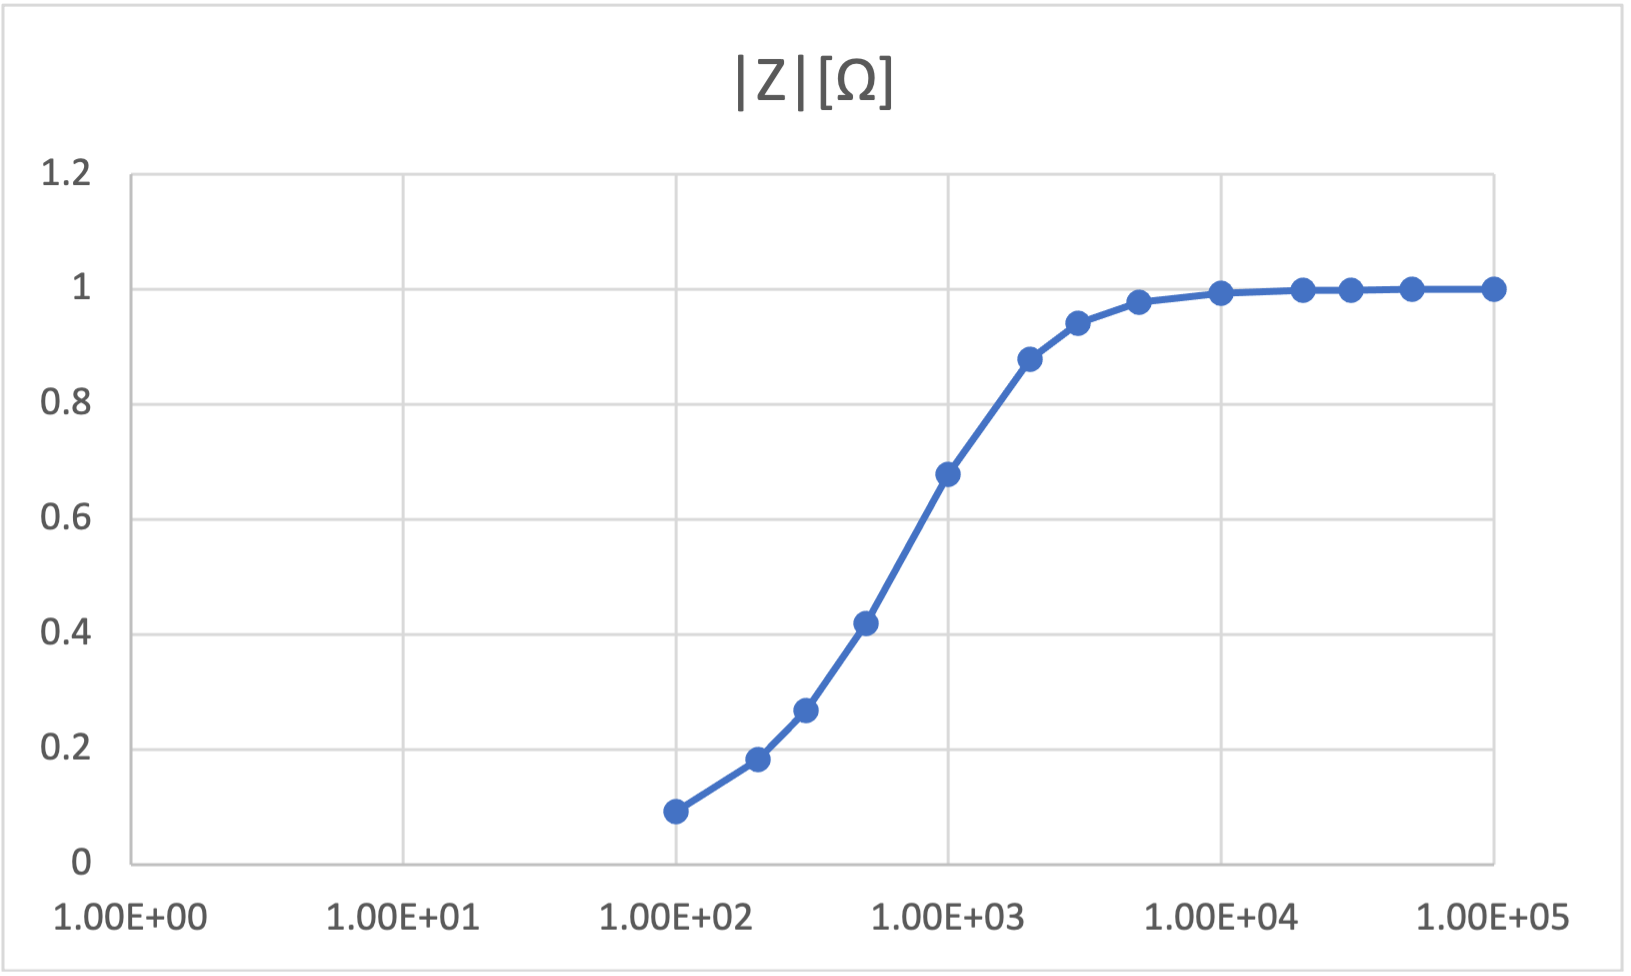
\includegraphics[height=7cm,width=10cm]{sekibun1.png}
  \caption{積分回路のゲインの周波数特性}
\end{center}
\end{figure}
\begin{figure}[H]
  \begin{center}
  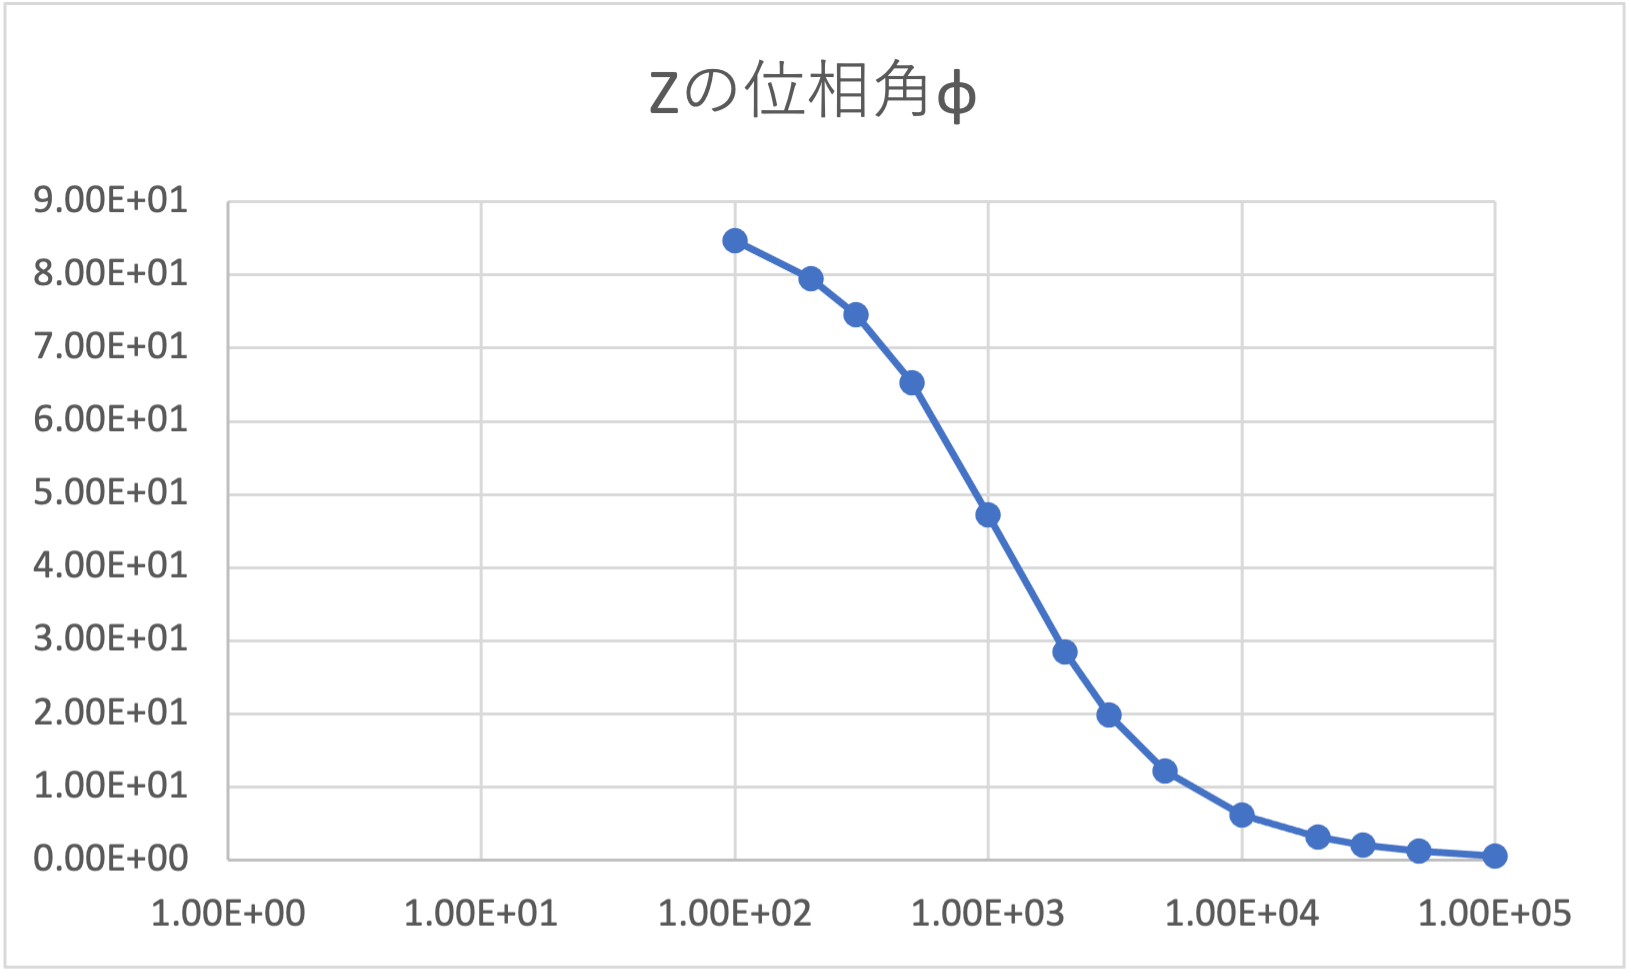
\includegraphics[height=7cm,width=10cm]{sekibun2.png}
  \caption{積分回路の位相差の周波数特性}
\end{center}
\end{figure}
となった.
つぎに微分回路のシュミレーション結果を表で示す.
\begin{table}[H]
  \label{biresult2}
  \begin{center}
    \caption{微分回路のシュミレーション結果}
    \begin{tabular}{cccc}
      周波数 & Zの常用対数の値 & Zの位相角φ & \textbar{Z}\textbar[Ω] \\ \hline
1.00E+02 & -2.07E+01 & 8.47E+01 & 0.091954113 \\
2.00E+02 & -1.48E+01 & 7.95E+01 & 0.181619115 \\
3.00E+02 & -1.15E+01 & 7.45E+01 & 0.26698022 \\
5.00E+02 & -7.55E+00 & 6.52E+01 & 0.419199127 \\
1.00E+03 & -3.37E+00 & 4.73E+01 & 0.678429497 \\
2.00E+03 & -1.12E+00 & 2.84E+01 & 0.879373317 \\
3.00E+03 & -5.32E-01 & 1.98E+01 & 0.940598149 \\
5.00E+03 & -1.99E-01 & 1.22E+01 & 0.977341011 \\
1.00E+04 & -5.06E-02 & 6.18E+00 & 0.994187798 \\
2.00E+04 & -1.27E-02 & 3.10E+00 & 0.998537398 \\
3.00E+04 & -5.65E-03 & 2.07E+00 & 0.999349162 \\
5.00E+04 & -2.04E-03 & 1.24E+00 & 0.999765552 \\
1.00E+05 & -5.09E-04 & 6.20E-01 & 0.999941372 \\

\end{tabular}
\end{center}
\end{table}
これをもとにゲインの周波数特性,位相差の周波数特性をそれぞれグラフにすると
\begin{figure}[H]
  \begin{center}
  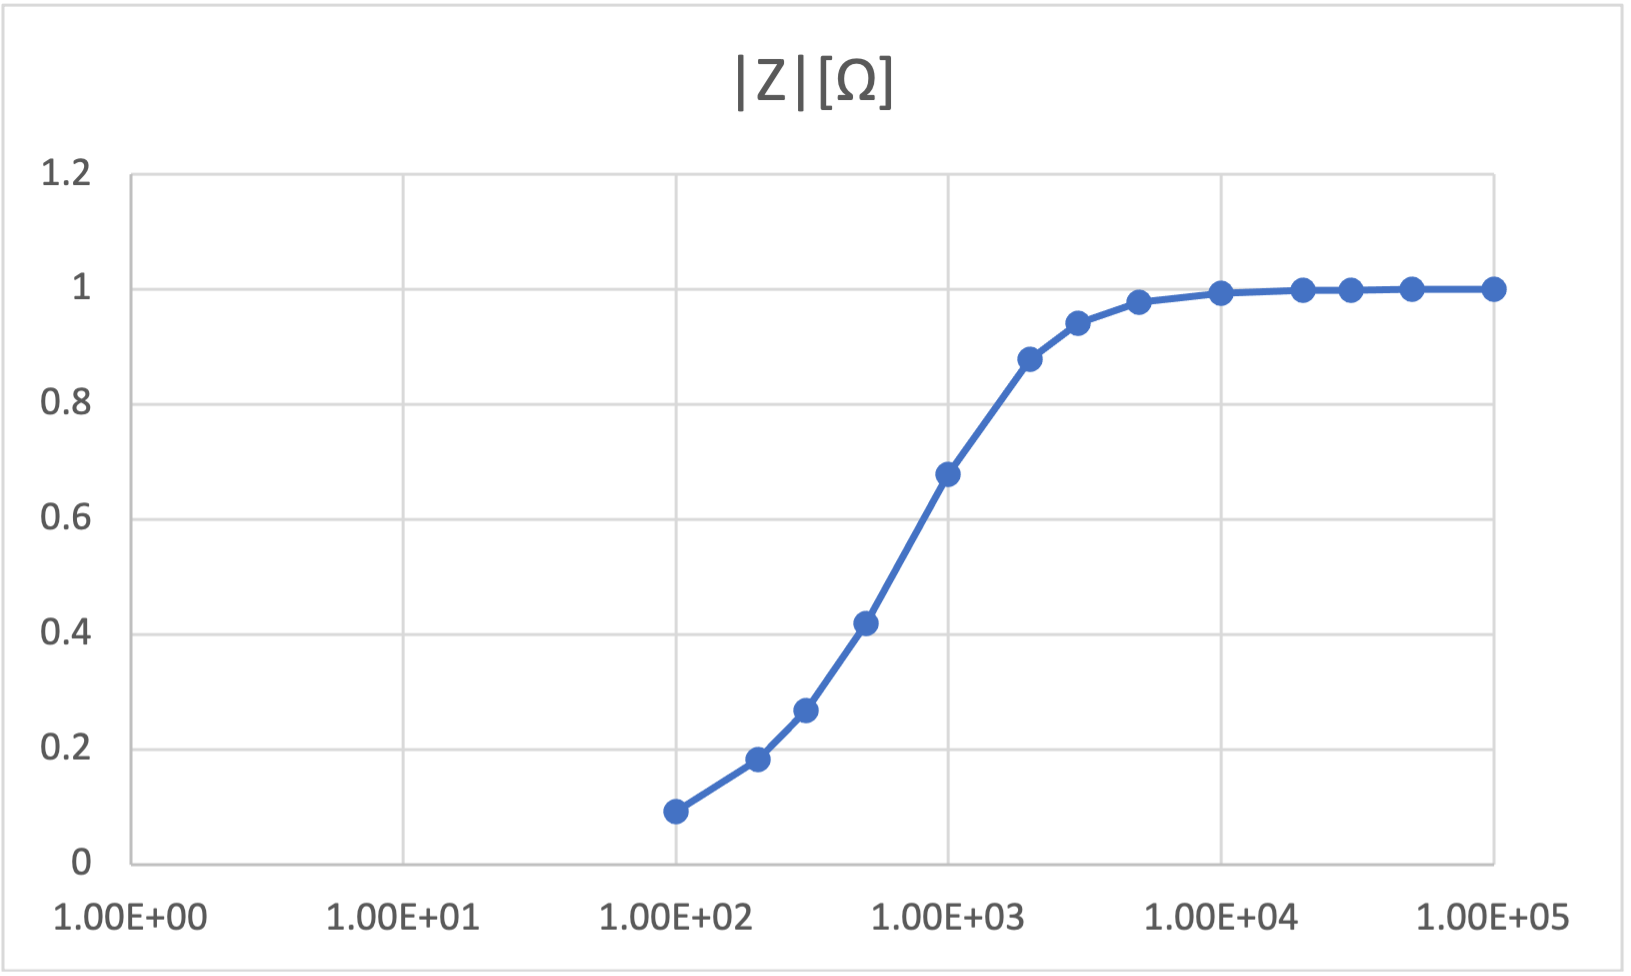
\includegraphics[height=7cm,width=10cm]{bibun1.png}
  \caption{微分回路のゲインの周波数特性}
\end{center}
\end{figure}
\begin{figure}[H]
  \begin{center}
  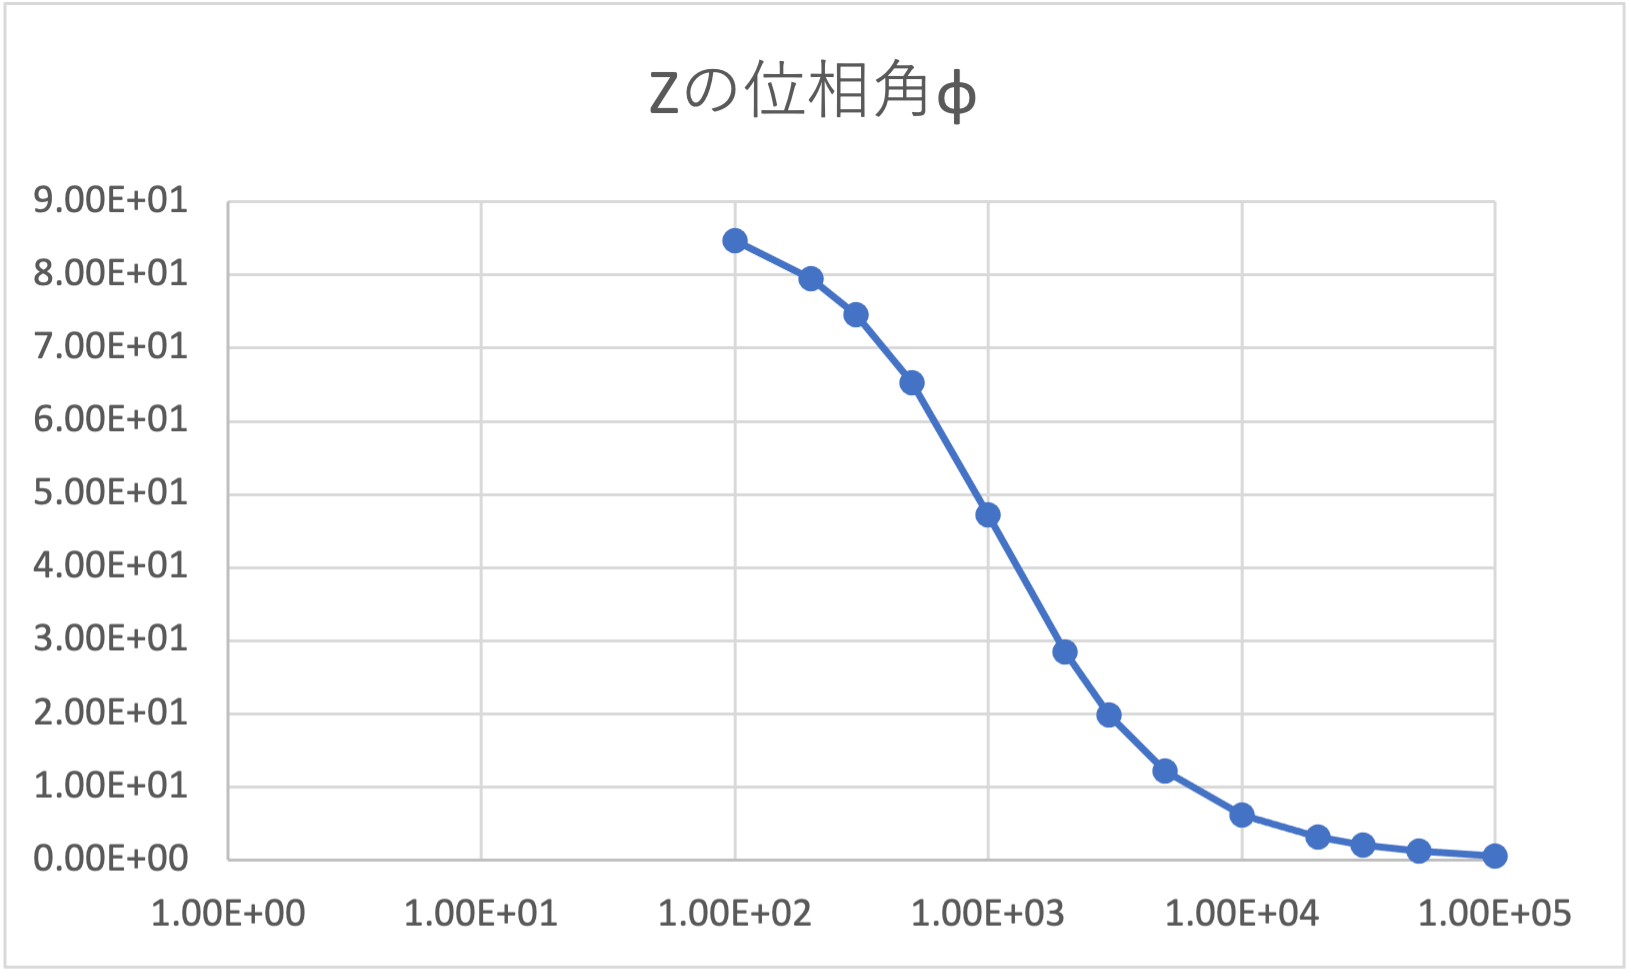
\includegraphics[height=7cm,width=10cm]{bibun2.png}
  \caption{微分回路の位相差の周波数特性}
\end{center}
\end{figure}
となった.
\subsection{積分回路の過渡応答}
積分回路の100kHz, 1kHz, 0.1kHz の時の過渡応答の実験結果のオシロスコープの画像をそれぞれ示す.
\begin{figure}[H]
  \begin{center}
  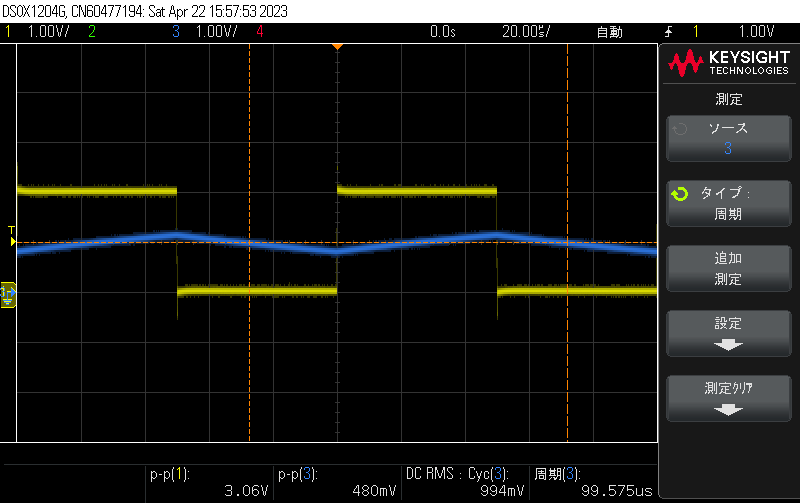
\includegraphics[height=7cm,width=10cm]{10khz.png}
  \caption{10kHz}
\end{center}
\end{figure}
\begin{figure}[H]
  \begin{center}
  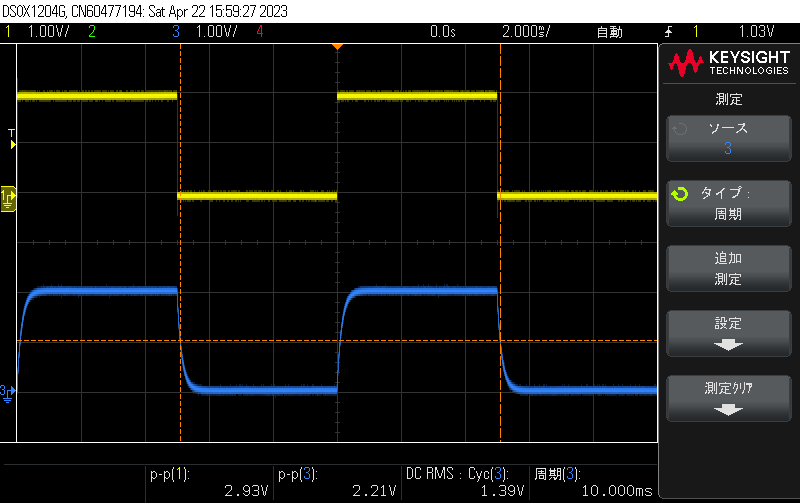
\includegraphics[height=7cm,width=10cm]{100hz.png}
  \caption{0.1kHz}
\end{center}
\end{figure}
\begin{figure}[H]
  \begin{center}
  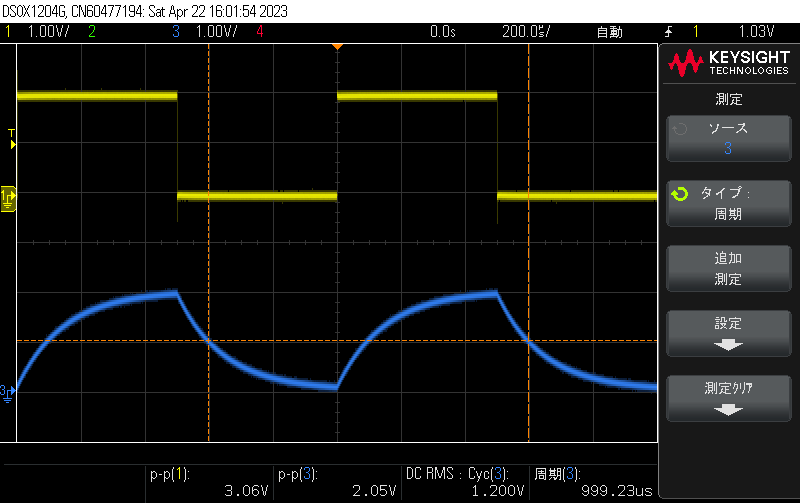
\includegraphics[height=7cm,width=10cm]{1khz.png}
  \caption{1kHz}
\end{center}
\end{figure}
次に測定条件1kHz,(\ref{tji})より時定数$1.468^{-4}[s]$のときの立ち上がりと立ち下がりの電圧のオシロスコープの画像をそれぞれ示す.
\begin{figure}[H]
  \begin{center}
  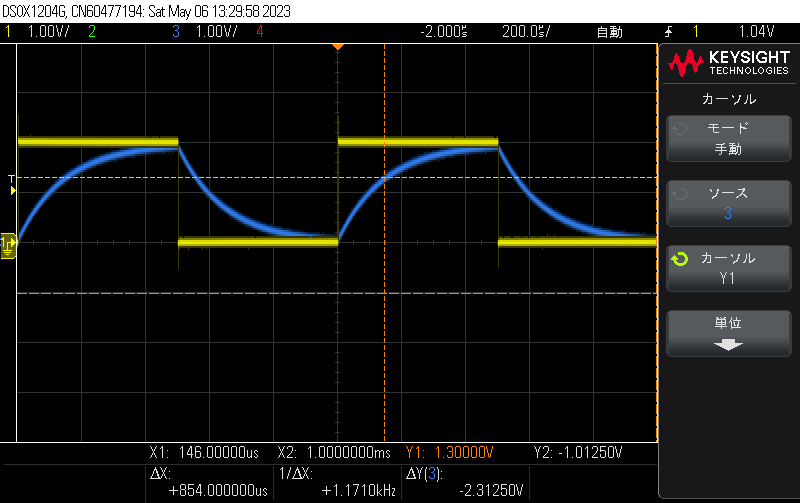
\includegraphics[height=7cm,width=10cm]{1khztatiagari.png}
  \caption{1kHz立ち上がり}
\end{center}
\end{figure}
\begin{figure}[H]
  \begin{center}
  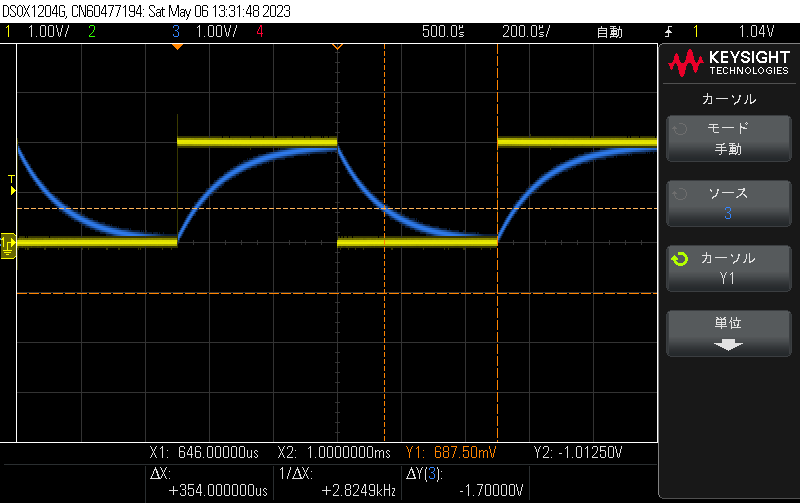
\includegraphics[height=7cm,width=10cm]{1khztatisagari.png}
  \caption{1kHz立ち下がり}
\end{center}
\end{figure}
\subsection{積分回路の周波数特性}
積分回路の周波数特性の実験結果を示していく.
実測値カットオフ周波数は1.078kHzとなった.それぞれの値を表に示していく.
\begin{table}[H]
  \label{res3}
  \begin{center}
    \caption{積分回路の周波数特性}
    \begin{tabularx}{\textwidth}{X|XXXXXX||XX}
      & 実測値 &  &  &  &  &  & 理論値(ESRの考慮なし) &  \\ \hline
      &  & 実効値 & 実効値 & 振幅比実測値 & 時間差 & 位相差実測値 & 振幅比理論値 & 位相差理論値 \\ \hline
     f [kHz] & Fgout [Vp-p] & vi (CH1) [mV] & vo (CH2) [mV] & 利得 [dB] & Δt [us] & 位相差 [deg.] & 振幅 [dB] & 位相差 [deg.] \\ \hline
     100 & 2 & 721  & 8.01  & -39.086  & -2.539  & -91.40  & -39.309  & -89.380  \\
     50 & 2 & 719  & 15.8  & -33.139  & -4.900  & -88.20  & -33.290  & -88.759  \\
     20 & 2 & 717  & 39.0  & -25.289  & -12.00  & -86.40  & -25.342  & -86.901  \\
     10 & 2 & 717  & 77.0  & -19.381  & -23.40  & -84.24  & -19.359  & -83.820  \\
     5 & 2 & 717  & 152  & -13.474  & -43.00  & -77.40  & -13.487  & -77.780  \\
     2 & 2 & 717  & 339  & -6.506  & -84.00  & -60.48  & -6.445  & -61.567  \\
     1.083 & 2 & 715  & 500  & -3.107  & -114.0  & -44.44  & -3.010  & -45.000  \\
     1.078 & 2 & 715  & 505  & -3.020  & -115.0  & -44.63  & -2.991  & -44.870  \\
     1 & 2 & 715  & 521  & -2.749  & -118.0  & -42.48  & -2.678  & -42.721  \\
     0.5 & 2 & 716  & 649  & -0.853  & -138.0  & -24.84  & -0.839  & -24.784  \\
     0.2 & 2 & 718  & 730  & 0.144  & -145.0  & -10.44  & -0.146  & -10.464  \\
     0.1 & 2 & 763  & 760  & -0.034  & -143.0  & -5.15  & -0.037  & -5.276  \\
     0.05 & 2 & 744  & 743  & -0.012  & -150.0  & -2.70  & -0.009  & -2.644  \\
    \end{tabularx}
  \end{center}
  \end{table}
  これらの値から利得とRC積分回路の位相差をそれぞれグラフにすると
  \begin{figure}[H]
    \begin{center}
    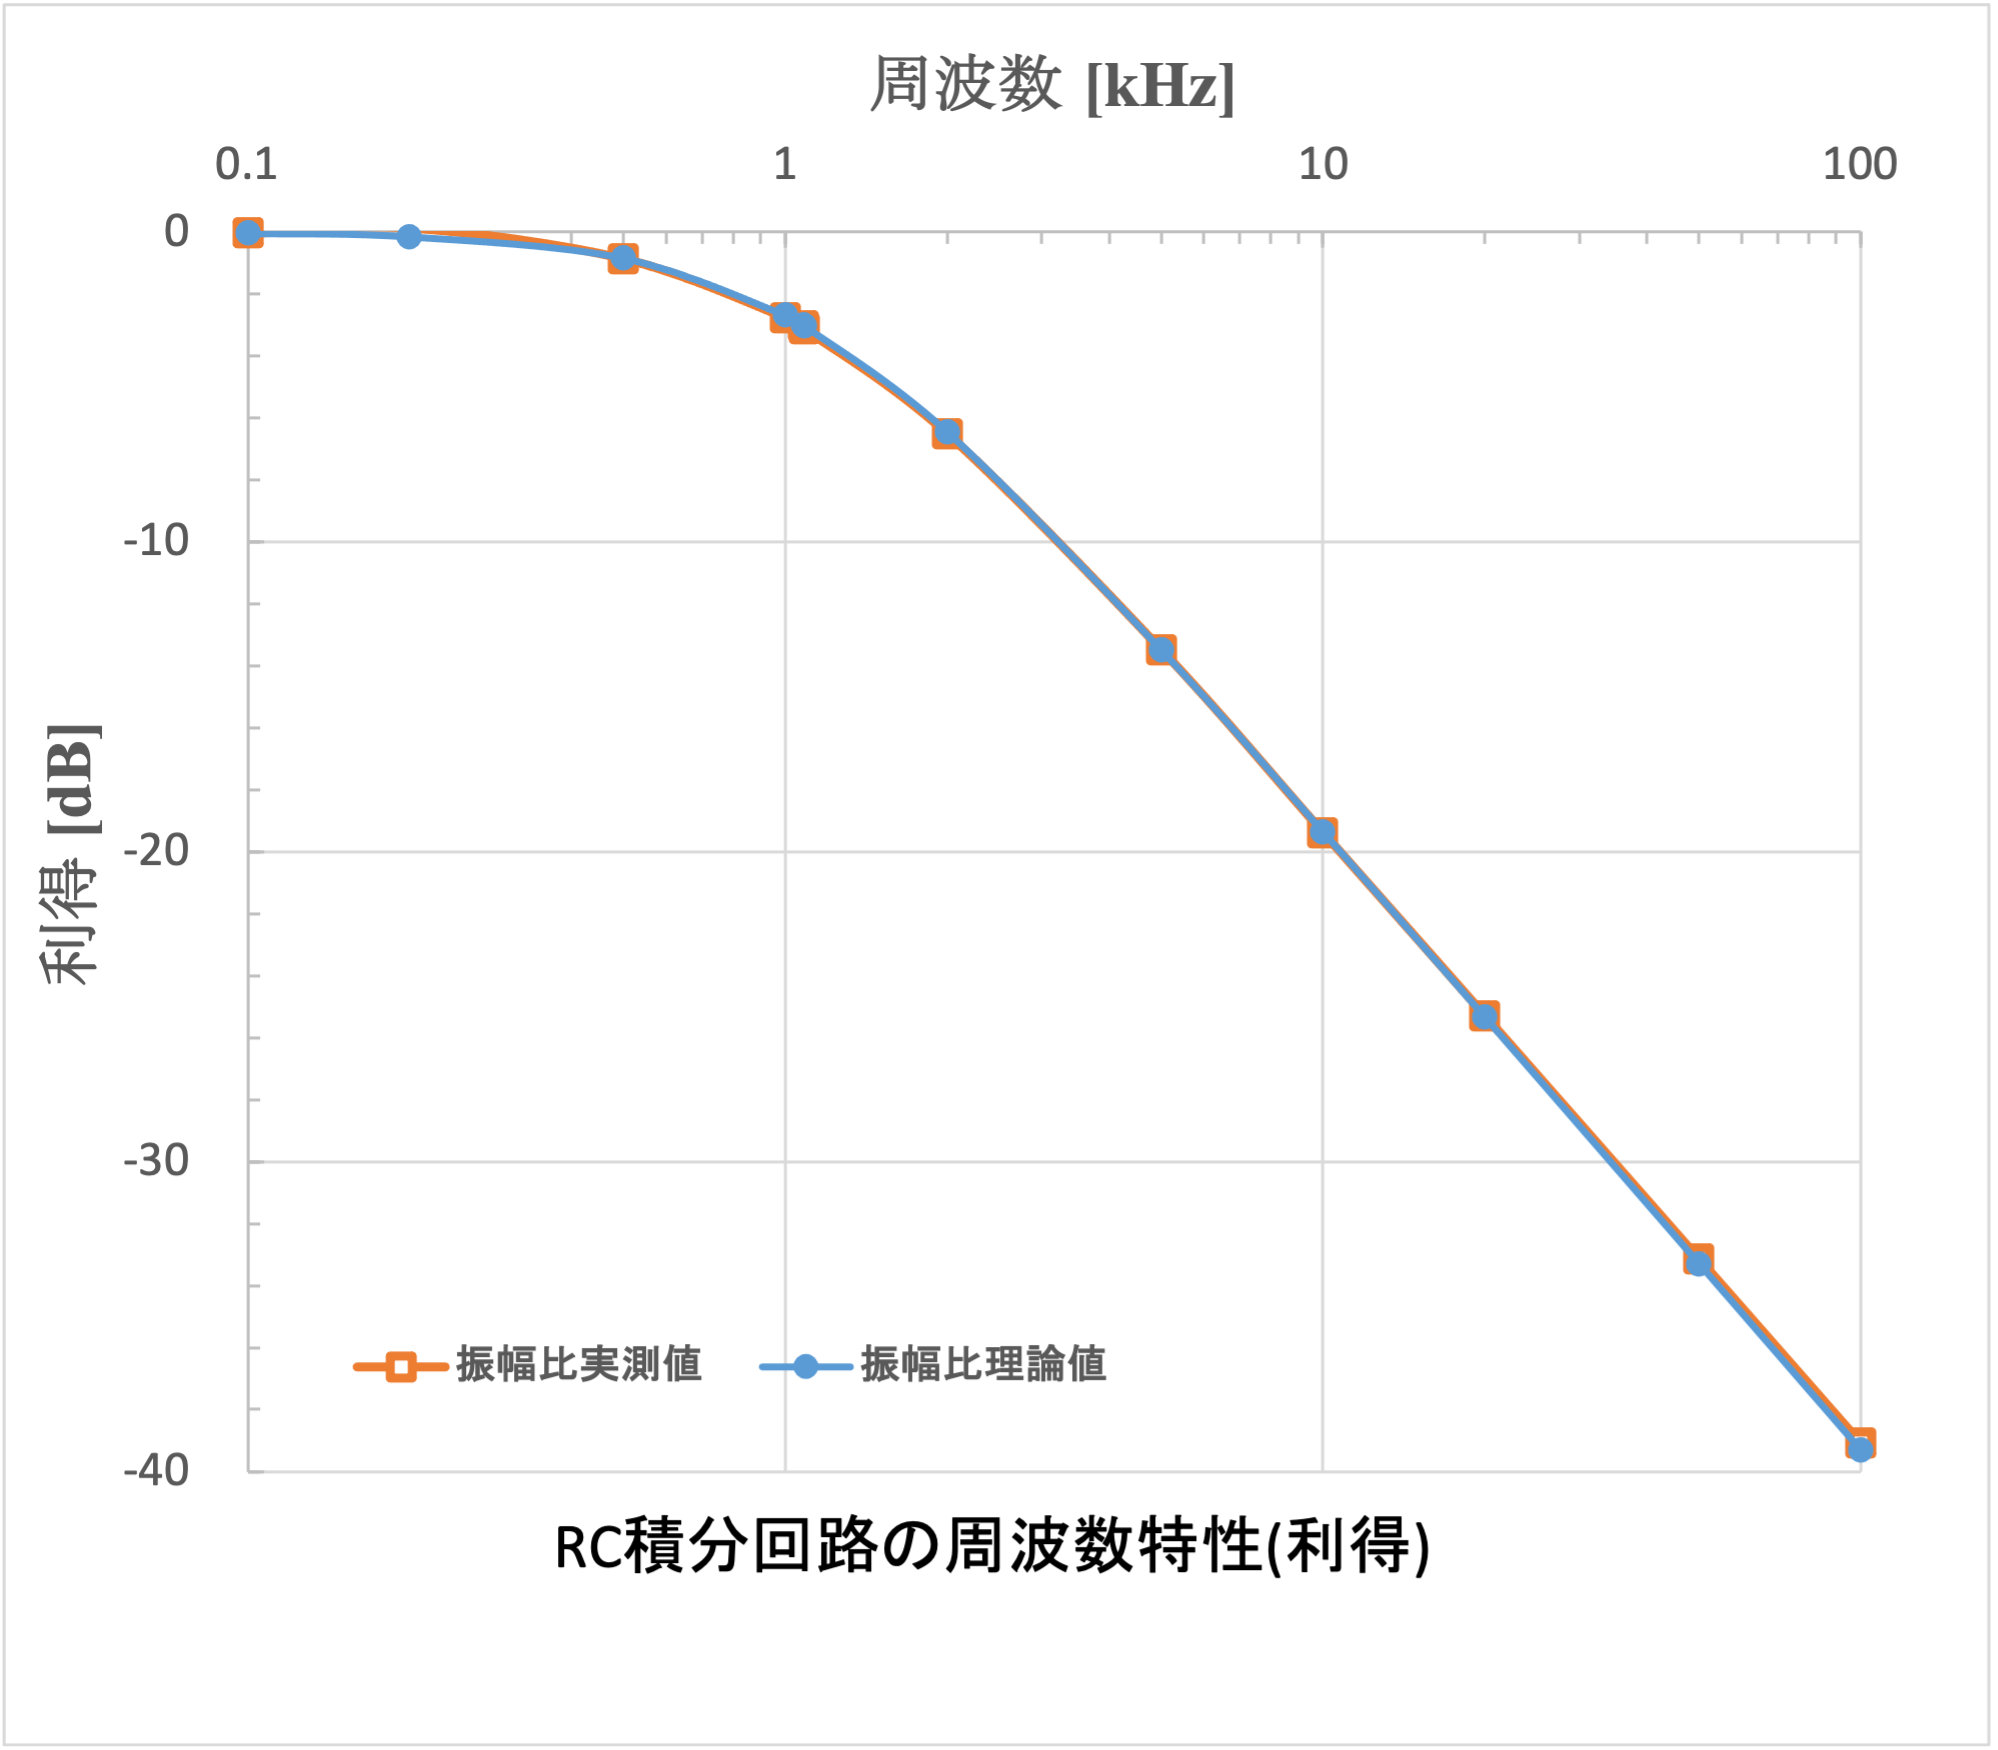
\includegraphics[height=7cm,width=10cm]{3-1.png}
    \caption{RC積分回路の周波数特性(利得)}
    \label{res3-1}
  \end{center}
  \end{figure}
  \begin{figure}[H]
    \begin{center}
    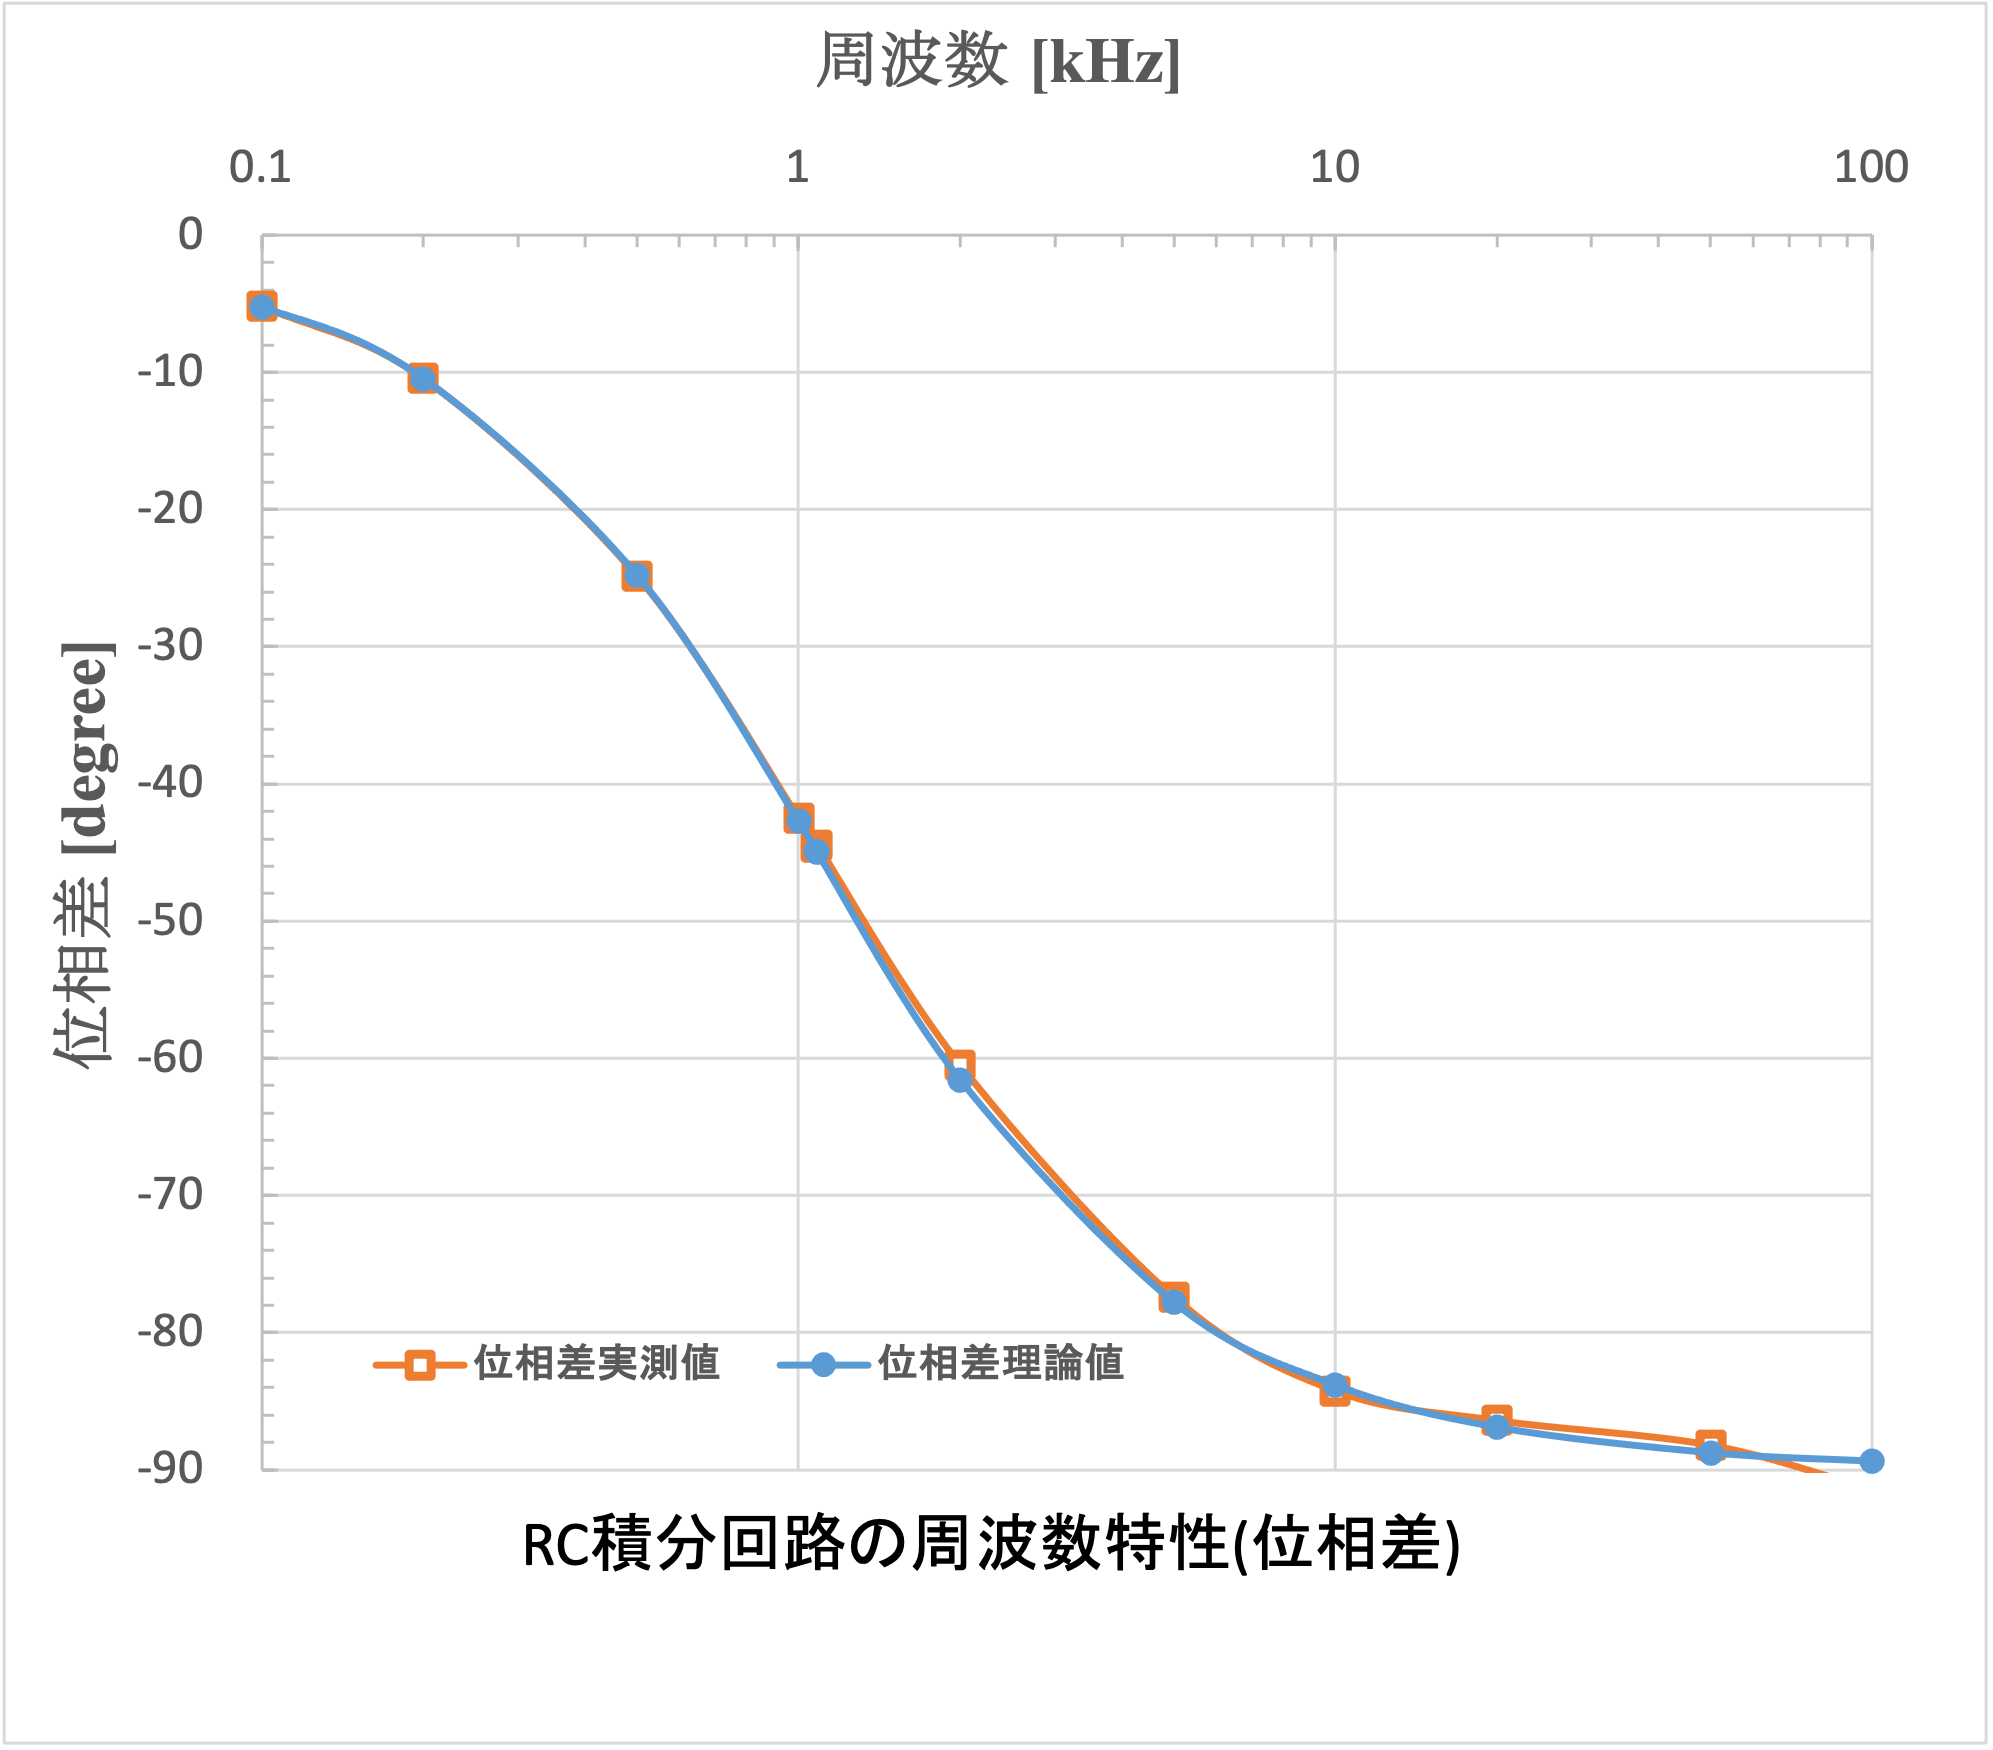
\includegraphics[height=7cm,width=10cm]{3-2.png}
    \caption{RC積分回路の周波数特性(位相差)}
    \label{res3-2}
  \end{center}
  \end{figure}
となった.
\section{考察}
\subsection{充電過程と放電過程において時定数の実測値と原理から導き出される理論値,シミュレーション結果の波形を比較し,その結果を定性的に報告する.}
時定数は(\ref{tj})より$1.468^{-4}$[s]となり,実測値と理論値がとても近いものとなった.
\subsection{RC回路の周波数特性について,ゲイン,位相ごとに理論式から得られるグラフと実測から得られるグラフを同一のグラフ内に書き記した上で,同一であった事柄と異なっていた事柄について考察する.}
理論値と実測値を表(\ref{res3})と利得のグラフ(\ref{res3-1}),位相差のグラフ(\ref{res3-2})を見たところ,大きくズレている値はほとんどなく,測定結果は正常なものと考えられる.また100kHzの高い周波数で誤差が多少大きくなっているのも,
高周波になるほど回路の浮遊容量や測定機の誤差が発生しやすくなるので許容できるものであると考えられる.
\section{まとめ}
積分回路と微分回路の特性をシュミレーションを用いた実験,積分回路のキャパシタ部の波形を観測し過渡応答を確認する実験,積分回路の出入力電圧と位相を測定する実験を行った.これらの実験を通して理論値に近い数字を測定したことによりオシロスコープ等実験器具を正しく使えていることがわかった.
また実験の目的であるRC直列回路への理解も多少深まった.

\begin{thebibliography}{9}
  \bibitem{a} 電気通信大学『アナログ回路実験』2023年,p1$\sim$3
  \bibitem{b}analogDialog, https://www.analog.com/jp/analog-dialogue/studentzone/studentzone-october-2018.html,「ADALM1000」で、SMUの基本を学ぶトピック10:ローパス・フィルタとハイパス・フィルタ
\end{thebibliography}
\end{document}
